\documentclass[10pt,aspectratio=169]{beamer}

% ---------- Theme ----------
\usetheme{metropolis}
\metroset{progressbar=frametitle}

\usepackage[T1]{fontenc}
\usepackage[utf8]{inputenc}
\usepackage{listings}
\usepackage{xcolor}
\usepackage{tikz}
\usepackage{hyperref}

% --- Logos on the title slide (top right) ---
% Place 'logo_fraunhofer.png' and 'logo_bremen.png' next to this .tex file.
\addtobeamertemplate{title page}{%
  \begin{tikzpicture}[remember picture,overlay]
    \node[anchor=north east,inner sep=0pt,xshift=-0.5cm,yshift=-0.4cm]
      at (current page.north east)
      {
\includegraphics[height=0.9cm]{assets/Logo MEVIS 14_mevis_rgb.png}};
    \node[anchor=north east,inner sep=0pt,xshift=-0.5cm,yshift=-1.7cm]
      at (current page.north east)
      {
\includegraphics[height=0.8cm]{assets/UHB_Logo_Englisch_Web_RGB.png}};
  \end{tikzpicture}%
}{}

% ---------- Colors for code ----------
\definecolor{codebg}{RGB}{245,245,245}
\definecolor{codekw}{RGB}{0,102,204}
\definecolor{codestr}{RGB}{163,21,21}
\definecolor{codecom}{RGB}{0,128,0}
\definecolor{codenum}{RGB}{120,120,120}

% ---------- Listings setup for Python ----------
\lstdefinestyle{pythonstyle}{
  language=Python,
  backgroundcolor=\color{codebg},
  basicstyle=\ttfamily\scriptsize,
  keywordstyle=\color{codekw}\bfseries,
  stringstyle=\color{codestr},
  commentstyle=\color{codecom}\itshape,
  numberstyle=\tiny\color{codenum},
  numbers=left,
  numbersep=6pt,
  showstringspaces=false,
  breaklines=true,
  breakatwhitespace=true,
  frame=single,
  rulecolor=\color{black!20},
  framexleftmargin=4pt,
  framexrightmargin=2pt,
  xleftmargin=12pt,
  tabsize=2,
  columns=fullflexible,
  keepspaces=true,
  morekeywords={as,with,True,False,None,self}
}
\lstset{style=pythonstyle}
\renewcommand{\section}[2][]{}
% \setbeamertemplate{section page}{}
\usepackage{courier}

% ---------- Title ----------
\title{Lung Segmentation using\\Marker-Controlled Watershed Transformation}
\subtitle{A walk-through of the Python implementation}
\author{Course Material presented by Horst Hahn regarding the ipynp on \href{https://www.kaggle.com/code/aadhavvignesh/lung-segmentation-by-marker-controlled-watershed}{kaggle.com by Aadhav Vignesh}}
\date{\today}

\begin{document}

\begin{frame}
  \titlepage
\end{frame}

\begin{frame}{Example 1}
\begin{figure}
    \centering
    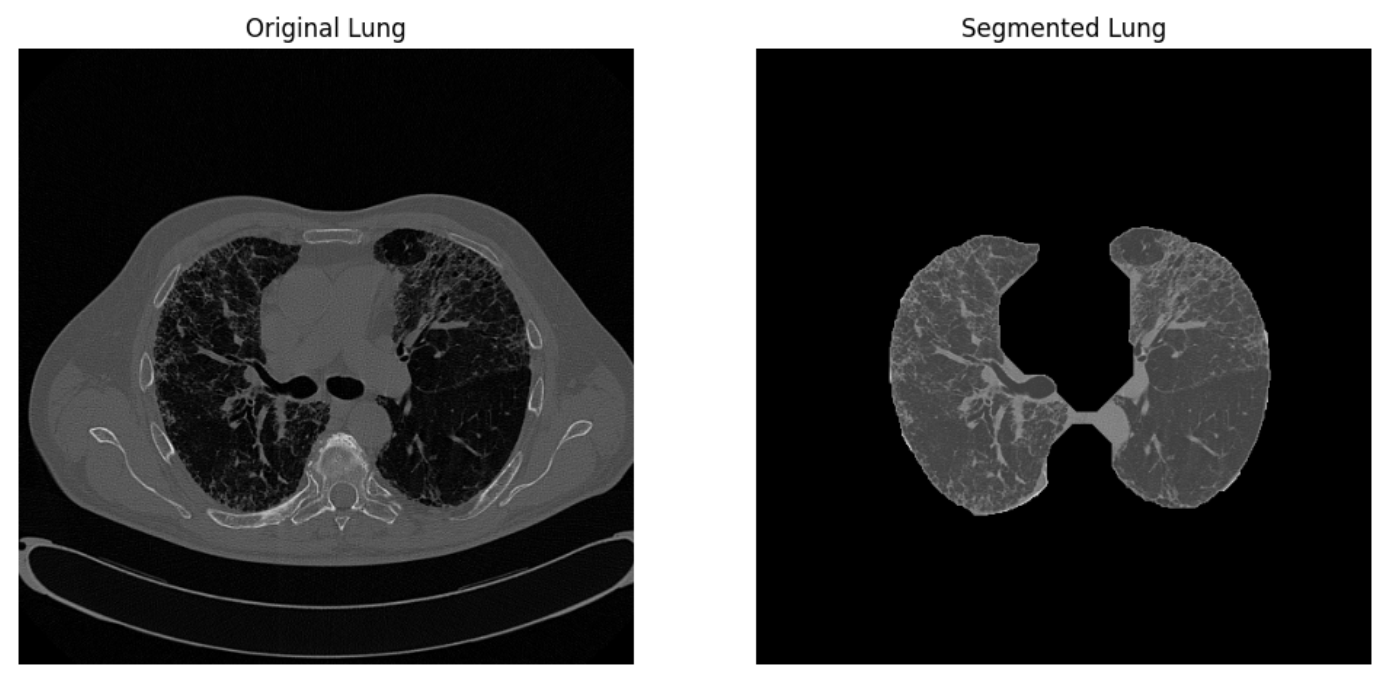
\includegraphics[width=1\linewidth]{lung-seg-watershed-example-24-10.png}
    \caption{Example input and output for patient 24, slice 10}
\end{figure}
\end{frame}

\begin{frame}{Example 2}
\begin{figure}
    \centering
    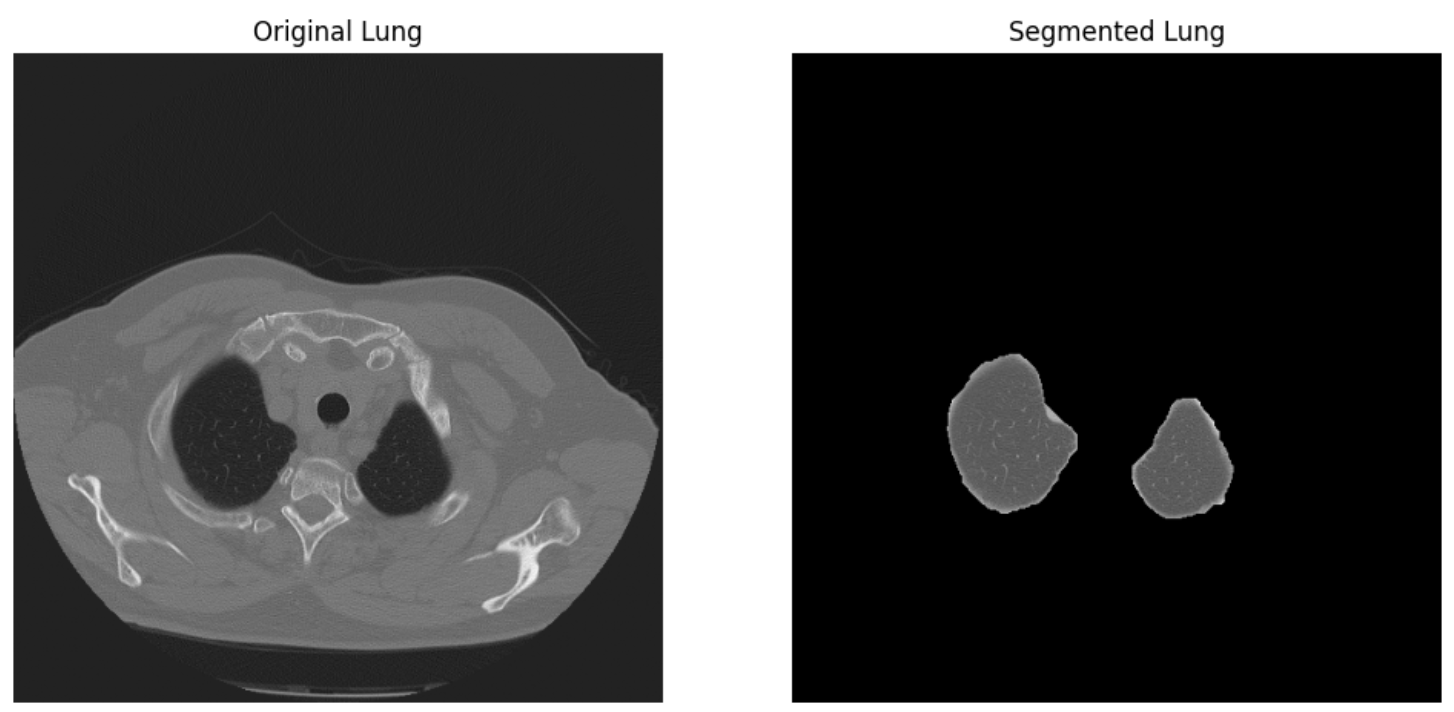
\includegraphics[width=1\linewidth]{lung-seg-watershed-example-23-30.png}
    \caption{Example input and output for patient 23, slice 30}
\end{figure}
\end{frame}

\begin{frame}{Example 3}
\begin{figure}
    \centering
    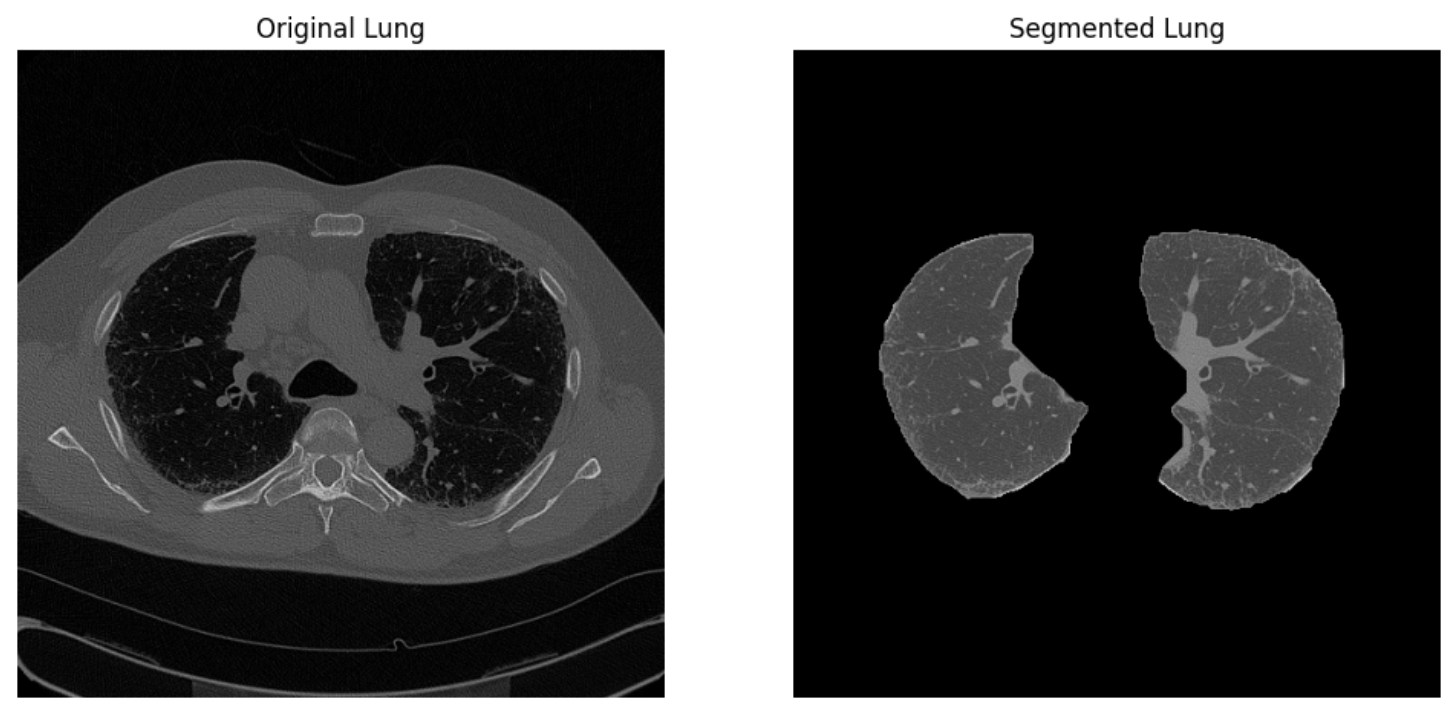
\includegraphics[width=1\linewidth]{lung-seg-watershed-example-22-120.png}
    \caption{Example input and output for patient 22, slice 120}
\end{figure}
\end{frame}

\begin{frame}{Overview}
  \begin{itemize}
    \item CT scans are stored as DICOM files with pixel values that map to tissue density.
    \item We want to isolate the lung tissue from the rest of the chest scan.
    \item Plain thresholding by Hounsfield Units picks up too much unwanted region.
    \item \textbf{Marker-controlled watershed} treats the image as a landscape and floods it from chosen seed points, giving a clean lung mask.
    \item The notebook walks through: loading scans, converting to HU, generating markers, computing the Sobel gradient, running watershed, and cleaning up the mask.
  \end{itemize}
\end{frame}

\section{Setup and imports}

\begin{frame}[fragile]{Installing and importing libraries}
\begin{columns}[T,onlytextwidth]
\begin{column}{0.42\textwidth}
\small
We install \texttt{pydicom}, the standard Python library for reading DICOM medical image files. The bang \texttt{!} runs the command in the system shell from inside a Jupyter notebook.\\[0.4em]
The imports cover everything we need:
\begin{itemize}
  \item \texttt{numpy}, \texttt{pandas} for arrays and tables
  \item \texttt{pydicom} to read CT scan files
  \item \texttt{scipy.ndimage} for image filters (Sobel, dilation, etc.)
  \item \texttt{skimage} for measurement and morphology
  \item \texttt{matplotlib} for plotting
  \item \texttt{time} to measure how long each step takes
\end{itemize}
\end{column}
\begin{column}{0.56\textwidth}
\begin{lstlisting}[firstnumber=last]
!pip install pydicom

%matplotlib inline

import numpy as np
import pandas as pd
import pydicom
import os
import scipy.ndimage as ndimage
from skimage import measure, morphology, segmentation
import matplotlib.pyplot as plt

import time
\end{lstlisting}
\end{column}
\end{columns}
\end{frame}

\section{Loading patient data}

\begin{frame}[fragile]{Listing the patients}
\begin{columns}[T,onlytextwidth]
\begin{column}{0.42\textwidth}
\small
The dataset is laid out so each patient gets one folder, and that folder contains the slices of one CT scan.\\[0.4em]
\texttt{os.listdir} returns all folder names in the input directory. Each name is a unique patient ID.\\[0.4em]
We sort the list so the order is reproducible and print the first five IDs to confirm everything is in place.\\[0.4em]
\textbf{Why sort?} Without sorting, the order depends on the filesystem and can change between runs.
\end{column}
\begin{column}{0.56\textwidth}
\begin{lstlisting}[firstnumber=last]
INPUT_FOLDER = '/kaggle/input/osic-pulmonary-fibrosis-progression/train/'

patients = os.listdir(INPUT_FOLDER)
patients.sort()

print("Some examples of patient IDs:")
print(",\n".join(patients[:5]))
\end{lstlisting}
\end{column}
\end{columns}
\end{frame}

\section{Reading a CT scan}

\begin{frame}[fragile]{The \texttt{load\_scan} function}
\begin{columns}[T,onlytextwidth]
\begin{column}{0.42\textwidth}
\small
Reads all DICOM slices for one patient and returns them as a sorted list.\\[0.4em]
\textbf{Step by step:}
\begin{itemize}
  \item List comprehension reads every file with \texttt{pydicom.read\_file}.
  \item Slices arrive in random order, so we sort by \texttt{InstanceNumber}, the slice index in the DICOM header.
  \item The slice thickness in mm is computed from the patient position. If that field is missing, we fall back to \texttt{SliceLocation} via \texttt{try/except}.
  \item We write the thickness back into every slice so it is available later.
\end{itemize}
\end{column}
\begin{column}{0.56\textwidth}
\begin{lstlisting}[firstnumber=last]
def load_scan(path):
    """
    Loads scans from a folder into a list.
    """
    slices = [pydicom.read_file(path + '/' + s)
              for s in os.listdir(path)]
    slices.sort(key=lambda x: int(x.InstanceNumber))

    try:
        slice_thickness = np.abs(
            slices[0].ImagePositionPatient[2]
            - slices[1].ImagePositionPatient[2])
    except:
        slice_thickness = np.abs(
            slices[0].SliceLocation
            - slices[1].SliceLocation)

    for s in slices:
        s.SliceThickness = slice_thickness

    return slices
\end{lstlisting}
\end{column}
\end{columns}
\end{frame}

\section{Hounsfield Units}

\begin{frame}[fragile]{Python syntax: list comprehension and \texttt{sort(key=...)}}
\begin{columns}[T,onlytextwidth]
\begin{column}{0.42\textwidth}
\small
\textbf{List comprehension} — a one-liner that builds a list. Read it as: for every \texttt{s} in the folder listing, call \texttt{pydicom.read\_file} on it, collect the results.\\[0.4em]
Equivalent to a \texttt{for} loop with \texttt{.append} but shorter.\\[0.4em]
\textbf{\texttt{sort(key=...)}} sorts in place. The \texttt{key} argument is a function that maps each element to a value to compare by.\\[0.4em]
\textbf{\texttt{lambda x: int(x.InstanceNumber)}} is an anonymous function: take \texttt{x}, return its \texttt{InstanceNumber} as an integer. The list ends up sorted by slice index.
\end{column}
\begin{column}{0.56\textwidth}
\begin{lstlisting}[stepnumber=0]
# List comprehension: build a list in one line
slices = [pydicom.read_file(path + '/' + s)
          for s in os.listdir(path)]

# Equivalent long form:
slices = []
for s in os.listdir(path):
    slices.append(pydicom.read_file(path + '/' + s))


# In-place sort with a key function
slices.sort(key=lambda x: int(x.InstanceNumber))

# Equivalent long form:
def slice_index(x):
    return int(x.InstanceNumber)
slices.sort(key=slice_index)
\end{lstlisting}
\end{column}
\end{columns}
\end{frame}

\begin{frame}{Hounsfield Units: the idea}
\begin{columns}[T,onlytextwidth]
\begin{column}{0.55\textwidth}
Hounsfield Units (HU) are a standardized way to express tissue density in CT scans.
\begin{itemize}
  \item Air: $\approx -1000$ HU
  \item Lung tissue: $-700$ to $-600$ HU
  \item Water: $0$ HU
  \item Blood, soft tissue: $+30$ to $+70$ HU
  \item Bone: $+700$ HU and above
\end{itemize}
The raw pixel values stored in a DICOM file are not HU yet. We convert them with a linear formula:
\[
  HU = m \cdot P + b
\]
where $m$ is the \texttt{RescaleSlope}, $b$ the \texttt{RescaleIntercept}, and $P$ the raw pixel.
\end{column}
\begin{column}{0.4\textwidth}
\centering
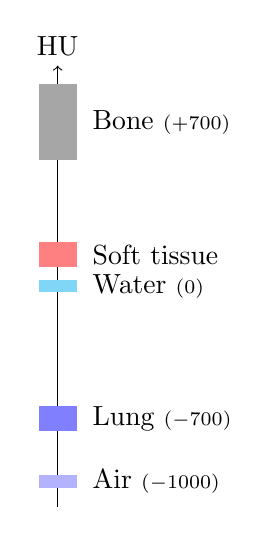
\begin{tikzpicture}[scale=0.8]
  \draw[->] (0,-3.5) -- (0,3.5) node[above] {HU};
  \fill[blue!30] (-0.3,-3.2) rectangle (0.3,-3) ; \node[right] at (0.4,-3.1) {Air \scriptsize($-1000$)};
  \fill[blue!50] (-0.3,-2.3) rectangle (0.3,-1.9); \node[right] at (0.4,-2.1) {Lung \scriptsize($-700$)};
  \fill[cyan!50] (-0.3,-0.1) rectangle (0.3,0.1) ; \node[right] at (0.4,0)    {Water \scriptsize($0$)};
  \fill[red!50]  (-0.3,0.3)  rectangle (0.3,0.7) ; \node[right] at (0.4,0.5)  {Soft tissue};
  \fill[gray!70] (-0.3,2.0)  rectangle (0.3,3.2) ; \node[right] at (0.4,2.6)  {Bone \scriptsize($+700$)};
\end{tikzpicture}
\end{column}
\end{columns}
\end{frame}

\begin{frame}[fragile]{The \texttt{get\_pixels\_hu} function}
\begin{columns}[T,onlytextwidth]
\begin{column}{0.42\textwidth}
\small
We stack all slices into a 3D NumPy array and convert raw pixels to HU.\\[0.4em]
\textbf{What each block does:}
\begin{itemize}
  \item \texttt{np.stack} builds a 3D array from the per-slice 2D arrays.
  \item Pixels with value $-2000$ come from outside the circular scan area (the corners of the square image). We set them to $0$.
  \item We apply $HU = m\cdot P + b$ using \texttt{RescaleSlope} and \texttt{RescaleIntercept} from the DICOM header.
  \item If the slope is exactly $1$ we skip the multiplication for speed.
\end{itemize}
\end{column}
\begin{column}{0.56\textwidth}
\begin{lstlisting}[firstnumber=42]
def get_pixels_hu(scans):
    """
    Converts raw images to Hounsfield Units.
    """
    image = np.stack([s.pixel_array for s in scans])
    image = image.astype(np.int16)

    # Outside the scanner: set to 0
    image[image == -2000] = 0

    # HU = m*P + b
    intercept = scans[0].RescaleIntercept
    slope = scans[0].RescaleSlope

    if slope != 1:
        image = slope * image.astype(np.float64)
        image = image.astype(np.int16)

    image += np.int16(intercept)

    return np.array(image, dtype=np.int16)
\end{lstlisting}
\end{column}
\end{columns}
\end{frame}

\section{Picking a sample slice}

\begin{frame}[fragile]{Python syntax: \texttt{np.stack} and boolean indexing}
\begin{columns}[T,onlytextwidth]
\begin{column}{0.42\textwidth}
\small
\textbf{\texttt{np.stack}} takes a list of arrays of the same shape and stacks them along a new axis. List of $N$ arrays of shape $(512, 512)$ becomes one array of shape $(N, 512, 512)$.\\[0.4em]
The list comprehension inside, \texttt{[s.pixel\_array for s in scans]}, just pulls the pixel array out of each DICOM slice.\\[0.4em]
\textbf{Boolean mask indexing} — \texttt{image == -2000} produces a boolean array of the same shape as \texttt{image}, \texttt{True} where the value is $-2000$. Using that boolean array as an index lets you read or write only those pixels.\\[0.4em]
The line \texttt{image[image == -2000] = 0} sets every $-2000$ pixel to zero in one step, no loop needed.
\end{column}
\begin{column}{0.56\textwidth}
\begin{lstlisting}[stepnumber=0]
# np.stack: combine many 2D arrays into one 3D array
image = np.stack([s.pixel_array for s in scans])

# Step by step:
# 1) [s.pixel_array for s in scans]
#    -> list of N arrays, each (512, 512)
# 2) np.stack(...)
#    -> single array of shape (N, 512, 512)


# Boolean mask indexing
image[image == -2000] = 0

# Step by step:
# 1) image == -2000
#    -> boolean array, True where pixel is -2000
# 2) image[<bool array>] = 0
#    -> assign 0 to every True position
\end{lstlisting}
\end{column}
\end{columns}
\end{frame}

\begin{frame}[fragile]{Loading one patient and showing a slice}
\begin{columns}[T,onlytextwidth]
\begin{column}{0.42\textwidth}
\small
We pick patient number 24 from the sorted list and run our two helper functions:
\begin{itemize}
  \item \texttt{load\_scan} returns the list of DICOM slices.
  \item \texttt{get\_pixels\_hu} converts them into one 3D NumPy array of HU values.
\end{itemize}
We then show slice 12 of the volume in grayscale.\\[0.4em]
This is the image we will segment in the rest of the notebook. Everything that follows operates on a single 2D slice of $512 \times 512$ pixels.
\end{column}
\begin{column}{0.56\textwidth}
\begin{lstlisting}[firstnumber=63]
test_patient_scans = load_scan(
    INPUT_FOLDER + patients[24])
test_patient_images = get_pixels_hu(
    test_patient_scans)

plt.imshow(test_patient_images[12], cmap='gray')
plt.title("Original Slice")
plt.show()
\end{lstlisting}
\end{column}
\end{columns}
\end{frame}

\section{Generating watershed markers}

\begin{frame}{Why markers?}
Watershed alone produces \textbf{over-segmentation}: every local minimum of the image becomes its own basin, and we end up with thousands of tiny regions.\\[0.6em]
The fix is \textbf{marker-controlled watershed}. We tell the algorithm where to start flooding by providing two markers:
\begin{itemize}
  \item an \textbf{internal marker} sitting inside the lung (the region of interest),
  \item an \textbf{external marker} sitting outside the lung (the background).
\end{itemize}
Combined into one \textbf{watershed marker} image, these seed the flooding process and keep it from spilling everywhere.
\end{frame}

\begin{frame}[fragile]{The \texttt{generate\_markers} function (1/2)}
\begin{columns}[T,onlytextwidth]
\begin{column}{0.42\textwidth}
\small
\textbf{Internal marker.} Start with a hard threshold: lung pixels are below $-400$ HU. That gives a binary mask.\\[0.4em]
The mask contains the lungs but also the air \emph{around} the body, which is below $-400$ HU as well and touches the image border. \texttt{clear\_border} removes any connected region that touches the border, wiping out that surrounding air and leaving the lungs (and a few small air pockets) inside.\\[0.4em]
\texttt{measure.label} assigns a unique integer ID to each connected region. We then keep only the two largest, since the lungs are the two biggest blobs of low-HU tissue. Anything smaller is air-pocket noise and gets zeroed out.
\end{column}
\begin{column}{0.56\textwidth}
\begin{lstlisting}[firstnumber=last]
def generate_markers(image):
    # Internal marker
    marker_internal = image < -400
    marker_internal = segmentation.clear_border(
        marker_internal)
    marker_internal_labels = measure.label(
        marker_internal)

    areas = [r.area for r in
             measure.regionprops(marker_internal_labels)]
    areas.sort()

    if len(areas) > 2:
        for region in measure.regionprops(
                marker_internal_labels):
            if region.area < areas[-2]:
                for coordinates in region.coords:
                    marker_internal_labels[
                        coordinates[0],
                        coordinates[1]] = 0

    marker_internal = marker_internal_labels > 0
\end{lstlisting}
\end{column}
\end{columns}
\end{frame}

\begin{frame}[fragile]{The \texttt{generate\_markers} function (2/2)}
\begin{columns}[T,onlytextwidth]
\begin{column}{0.42\textwidth}
\small
\textbf{External marker.} We dilate the internal marker twice with different radii (10 and 55 iterations) and take the XOR. The result is a ring around the lungs: definitely background, but not too far away.\\[0.4em]
\textbf{Watershed marker.} Combine both into one labeled image:
\begin{itemize}
  \item internal marker $\to$ value $255$ (lung seeds)
  \item external marker $\to$ value $128$ (background seeds)
\end{itemize}
The flooding will start from these seeds and meet at the lung border.
\end{column}
\begin{column}{0.56\textwidth}
\begin{lstlisting}[firstnumber=last]
    # External marker
    external_a = ndimage.binary_dilation(
        marker_internal, iterations=10)
    external_b = ndimage.binary_dilation(
        marker_internal, iterations=55)
    marker_external = external_b ^ external_a

    # Watershed marker
    marker_watershed = np.zeros(
        (512, 512), dtype=np.int)
    marker_watershed += marker_internal * 255
    marker_watershed += marker_external * 128

    return (marker_internal,
            marker_external,
            marker_watershed)
\end{lstlisting}
\end{column}
\end{columns}
\end{frame}

\begin{frame}[fragile]{Python syntax: writing into an array via coordinates, and XOR}
\begin{columns}[T,onlytextwidth]
\begin{column}{0.42\textwidth}
\small
\textbf{Region coordinates loop.} \texttt{regionprops} gives one object per connected region. Each region's \texttt{.coords} is an $(N, 2)$ array of $(\text{row}, \text{col})$ pairs. The nested loop walks every pixel of small regions and writes 0 into the labels array, effectively erasing them.\\[0.4em]
A vectorized version using fancy indexing would be faster, but the explicit loop is easier to read.\\[0.4em]
\textbf{XOR on boolean arrays.} The \texttt{\textasciicircum} operator, applied to two boolean NumPy arrays, returns \texttt{True} where exactly one of them is true.\\[0.4em]
\texttt{external\_b \textasciicircum\ external\_a} is the bigger dilated mask minus the smaller one — a ring-shaped region.
\end{column}
\begin{column}{0.56\textwidth}
\begin{lstlisting}[stepnumber=0]
# Writing zeros into an array via coordinate pairs
for region in measure.regionprops(labels):
    if region.area < threshold:
        for coordinates in region.coords:
            labels[coordinates[0],
                   coordinates[1]] = 0

# coordinates is a length-2 array: [row, col]
# labels[row, col] = 0 erases that pixel


# XOR on boolean arrays: ring = outer - inner
marker_external = external_b ^ external_a

# external_a: dilated 10 iterations  (small disk)
# external_b: dilated 55 iterations  (big disk)
# XOR is True where b is True but a is False
#   -> a hollow ring around the lungs
\end{lstlisting}
\end{column}
\end{columns}
\end{frame}

\begin{frame}[fragile]{Visualizing the three markers}
\begin{columns}[T,onlytextwidth]
\begin{column}{0.42\textwidth}
\small
Quick sanity check. We run \texttt{generate\_markers} on slice 12 and plot the three returned images side by side:
\begin{itemize}
  \item the internal marker (the two lung blobs),
  \item the external marker (the ring around them),
  \item the combined watershed marker.
\end{itemize}
The \texttt{subplots} call with \texttt{sharey=True} keeps all three images aligned vertically.\\[0.4em]
\texttt{axis('off')} hides the tick marks since they are not meaningful for image data.
\end{column}
\begin{column}{0.56\textwidth}
\begin{lstlisting}[firstnumber=109]
test_patient_internal, \
test_patient_external, \
test_patient_watershed = generate_markers(
    test_patient_images[12])

f, (ax1, ax2, ax3) = plt.subplots(
    1, 3, sharey=True, figsize=(15,15))

ax1.imshow(test_patient_internal, cmap='gray')
ax1.set_title("Internal Marker")
ax1.axis('off')

ax2.imshow(test_patient_external, cmap='gray')
ax2.set_title("External Marker")
ax2.axis('off')

ax3.imshow(test_patient_watershed, cmap='gray')
ax3.set_title("Watershed Marker")
ax3.axis('off')

plt.show()
\end{lstlisting}
\end{column}
\end{columns}
\end{frame}

\section{The full segmentation pipeline}

\begin{frame}[fragile]{Setup: timing lists}
\begin{columns}[T,onlytextwidth]
\begin{column}{0.42\textwidth}
\small
Before the main segmentation function we create two empty lists. They will collect:
\begin{itemize}
  \item the wall-clock time of each call to \texttt{seperate\_lungs},
  \item a label for the run (e.g. ``3 iterations'').
\end{itemize}
Later we will plot computation time vs. number of iterations to see how the parameter affects performance.\\[0.4em]
A tiny but useful pattern: keep your benchmarking state in lists at module level, append on every call, and visualize at the end.
\end{column}
\begin{column}{0.56\textwidth}
\begin{lstlisting}[firstnumber=last]
# Lists to store computation times
# and iterations
computation_times = []
iteration_titles = []
\end{lstlisting}
\end{column}
\end{columns}
\end{frame}

\begin{frame}[fragile]{\texttt{seperate\_lungs} (1/4): markers and Sobel gradient}
\begin{columns}[T,onlytextwidth]
\begin{column}{0.42\textwidth}
\small
The main pipeline. It takes one slice and returns the segmented lung plus several intermediate images.\\[0.4em]
\textbf{Sobel gradient.} The Sobel operator approximates the spatial derivative of the image. It returns large values at edges and near zero in flat regions.\\[0.4em]
We compute it along $x$ and $y$, then take the magnitude $\sqrt{G_x^2 + G_y^2}$ via \texttt{np.hypot}, and normalize to $[0, 255]$.\\[0.4em]
This gradient image is the elevation map the watershed will flood.
\end{column}
\begin{column}{0.56\textwidth}
\begin{lstlisting}[firstnumber=last]
def seperate_lungs(image, iterations=1):
    start = time.time()

    marker_internal, marker_external, \
        marker_watershed = generate_markers(image)

    # Sobel gradient
    sobel_filtered_dx = ndimage.sobel(image, 1)
    sobel_filtered_dy = ndimage.sobel(image, 0)
    sobel_gradient = np.hypot(
        sobel_filtered_dx, sobel_filtered_dy)
    sobel_gradient *= 255.0 / np.max(sobel_gradient)
\end{lstlisting}
\end{column}
\end{columns}
\end{frame}

\begin{frame}[fragile]{\texttt{seperate\_lungs} (2/4): watershed and outline}
\begin{columns}[T,onlytextwidth]
\begin{column}{0.42\textwidth}
\small
\textbf{Watershed.} We feed the Sobel gradient (the landscape) and the watershed marker (the seed regions) to \texttt{morphology.watershed}. The result is a labeled image: each pixel is tagged with the basin it belongs to.\\[0.4em]
\textbf{Outline.} A morphological gradient with a $3 \times 3$ structuring element returns the difference between the local max and min, which highlights the edges between basins. Casting it to \texttt{bool} gives a clean binary outline of the lung border.
\end{column}
\begin{column}{0.56\textwidth}
\begin{lstlisting}[firstnumber=last]
    # Watershed segmentation
    watershed = morphology.watershed(
        sobel_gradient, marker_watershed)

    # Reduce to outlines
    outline = ndimage.morphological_gradient(
        watershed, size=(3,3))
    outline = outline.astype(bool)
\end{lstlisting}
\end{column}
\end{columns}
\end{frame}

\begin{frame}[fragile]{\texttt{seperate\_lungs} (3/4): black top-hat}
\begin{columns}[T,onlytextwidth]
\begin{column}{0.42\textwidth}
\small
\textbf{Black top-hat.} The lung outline so far is mostly correct, but small dark structures (vessels, bronchi) right at the lung border are missed.\\[0.4em]
The black top-hat is defined as $\text{closing}(I) - I$. It returns small dark regions that fit inside the structuring element. Adding it to the outline pulls those missing border pieces into the mask.\\[0.4em]
We use a disk-shaped structuring element. \texttt{iterate\_structure} grows the disk with the \texttt{iterations} parameter, controlling how aggressive the cleanup is.
\end{column}
\begin{column}{0.56\textwidth}
\begin{lstlisting}[firstnumber=last]
    # Structuring element (disk-ish)
    blackhat_struct = [[0,0,1,1,1,0,0],
                       [0,1,1,1,1,1,0],
                       [1,1,1,1,1,1,1],
                       [1,1,1,1,1,1,1],
                       [1,1,1,1,1,1,1],
                       [0,1,1,1,1,1,0],
                       [0,0,1,1,1,0,0]]

    blackhat_struct = ndimage.iterate_structure(
        blackhat_struct, iterations)

    # Apply black top-hat to the outline
    outline += ndimage.black_tophat(
        outline, structure=blackhat_struct)
\end{lstlisting}
\end{column}
\end{columns}
\end{frame}

\begin{frame}[fragile]{\texttt{seperate\_lungs} (4/4): final mask and segmentation}
\begin{columns}[T,onlytextwidth]
\begin{column}{0.42\textwidth}
\small
\textbf{Lung filter.} Combine the internal marker with the cleaned outline using OR. A binary closing with a $5 \times 5$ kernel fills small gaps so the mask is solid.\\[0.4em]
\textbf{Segmentation.} \texttt{np.where} keeps the original HU values where the lung filter is true and replaces everything else with $-2000$ (clearly outside the body).\\[0.4em]
At the end we record the elapsed time and a label, then return all five images so the caller can inspect each step.
\end{column}
\begin{column}{0.56\textwidth}
\begin{lstlisting}[firstnumber=last]
    # Final lung filter
    lungfilter = np.bitwise_or(
        marker_internal, outline)
    lungfilter = ndimage.morphology.binary_closing(
        lungfilter,
        structure=np.ones((5,5)),
        iterations=3)

    # Segment the lung
    segmented = np.where(
        lungfilter == 1,
        image,
        -2000*np.ones((512, 512)))

    end = time.time()
    computation_times.append(end - start)
    iteration_titles.append(
        "{num} iterations".format(num=iterations))

    return (segmented, lungfilter, outline,
            watershed, sobel_gradient)
\end{lstlisting}
\end{column}
\end{columns}
\end{frame}

\section{Benchmark and visualization}

\begin{frame}[fragile]{Python syntax: \texttt{np.where} and multi-line tuple unpacking}
\begin{columns}[T,onlytextwidth]
\begin{column}{0.42\textwidth}
\small
\textbf{\texttt{np.where(cond, a, b)}} works element-wise: where \texttt{cond} is true, take the value from \texttt{a}, otherwise from \texttt{b}. All three must be broadcastable to the same shape.\\[0.4em]
In the segmentation step we keep the original HU value where the lung mask is true, and write $-2000$ everywhere else. The right-hand side \texttt{-2000*np.ones((512,512))} creates a $512 \times 512$ array filled with $-2000$.\\[0.4em]
\textbf{Multi-line tuple unpacking.} The function returns five values, packed into a tuple. We unpack into five names. The backslashes \texttt{\textbackslash} at the end of lines tell Python that the statement continues on the next line, so we can format the assignment vertically for readability.
\end{column}
\begin{column}{0.56\textwidth}
\begin{lstlisting}[stepnumber=0]
# np.where: element-wise if/else
segmented = np.where(
    lungfilter == 1,           # condition
    image,                     # value if True
    -2000*np.ones((512, 512))) # value if False

# At each pixel:
#   if lungfilter == 1: keep image[pixel]
#   else:               write -2000


# Multi-line unpacking with line continuations
test_segmented, \
test_lungfilter, \
test_outline, \
test_watershed, \
test_sobel_gradient = seperate_lungs(
    test_patient_images[12], itrs)

# Same as one long line, just easier to read
\end{lstlisting}
\end{column}
\end{columns}
\end{frame}

\begin{frame}[fragile]{Running with 1 to 8 iterations}
\begin{columns}[T,onlytextwidth]
\begin{column}{0.42\textwidth}
\small
A simple loop that calls \texttt{seperate\_lungs} eight times with iteration counts from $1$ to $8$.\\[0.4em]
On each call:
\begin{itemize}
  \item the function runs the full pipeline,
  \item appends the elapsed time to \texttt{computation\_times},
  \item appends a label to \texttt{iteration\_titles}.
\end{itemize}
The last call also overwrites the test variables, so afterwards \texttt{test\_segmented} etc. hold the result of the most recent run (8 iterations).
\end{column}
\begin{column}{0.56\textwidth}
\begin{lstlisting}[firstnumber=190]
for itrs in range(1, 9):
    test_segmented, \
    test_lungfilter, \
    test_outline, \
    test_watershed, \
    test_sobel_gradient = seperate_lungs(
        test_patient_images[12], itrs)
\end{lstlisting}
\end{column}
\end{columns}
\end{frame}

\begin{frame}[fragile]{Plotting iterations vs. time}
\begin{columns}[T,onlytextwidth]
\begin{column}{0.42\textwidth}
\small
We turn the two lists into a dict and plot a bar chart with Plotly.\\[0.4em]
\textbf{Color trick.} A list of eight identical dark-blue colors, then we overwrite index 0 with red. That way the default run (1 iteration) is highlighted and the rest stay neutral.\\[0.4em]
\texttt{texttemplate='\%\{y:.3s\}'} formats the bar labels with engineering notation (e.g. \texttt{120m} for 0.12\,s).\\[0.4em]
The chart tells us how the iteration count drives runtime, which helps pick a sensible default.
\end{column}
\begin{column}{0.56\textwidth}
\begin{lstlisting}[firstnumber=last]
itr_dict = {
  'Iterations': iteration_titles,
  'Computation Times (in seconds)':
      computation_times}
colors = ['#30336b'] * 8
colors[0] = '#eb4d4b'
import plotly.express as px
import plotly.graph_objects as go
fig = go.Figure(data=[go.Bar(
    x=itr_dict['Iterations'],
    y=itr_dict['Computation Times (in seconds)'],
    marker_color=colors)])
fig.update_traces(
    texttemplate='%{y:.3s}',
    textposition='outside')
fig.update_layout(
    title='Iterations vs Computation Times',
    yaxis=dict(
        title='Computation Times (in seconds)',
        titlefont_size=16,
        tickfont_size=14),
    autosize=False, width=800, height=800)
fig.show()
\end{lstlisting}
\end{column}
\end{columns}
\end{frame}

\begin{frame}[fragile]{Sobel gradient and watershed result}
\begin{columns}[T,onlytextwidth]
\begin{column}{0.42\textwidth}
\small
First inspection of the intermediate results.\\[0.4em]
\textbf{Left:} the Sobel gradient. Bright lines mark edges in the original image, dark areas are flat regions. This is the surface the watershed floods.\\[0.4em]
\textbf{Right:} the watershed labels. Each region is filled with one constant value, so we see the partition into basins. The lung interior is one big region.\\[0.4em]
Comparing them shows how the gradient guided the flooding.
\end{column}
\begin{column}{0.56\textwidth}
\begin{lstlisting}[firstnumber=last]
f, (ax1, ax2) = plt.subplots(
    1, 2, sharey=True, figsize=(12, 12))

ax1.imshow(test_sobel_gradient, cmap='gray')
ax1.set_title("Sobel Gradient")
ax1.axis('off')

ax2.imshow(test_watershed, cmap='gray')
ax2.set_title("Watershed")
ax2.axis('off')

plt.show()
\end{lstlisting}
\end{column}
\end{columns}
\end{frame}

\begin{frame}[fragile]{Outline, filter, and segmented lung}
\begin{columns}[T,onlytextwidth]
\begin{column}{0.42\textwidth}
\small
Three more steps of the pipeline shown in one figure:
\begin{itemize}
  \item \textbf{Lung outline}: the binary edge map after black top-hat.
  \item \textbf{Lung filter}: the closed binary mask of the full lung region.
  \item \textbf{Segmented lung}: the original HU values masked by the lung filter.
\end{itemize}
This is how the pipeline looks from raw edges to a usable lung region.
\end{column}
\begin{column}{0.56\textwidth}
\begin{lstlisting}[firstnumber=last]
f, (ax1, ax2, ax3) = plt.subplots(
    1, 3, sharey=True, figsize=(12, 12))

ax1.imshow(test_outline, cmap='gray')
ax1.set_title("Lung Outline")
ax1.axis('off')

ax2.imshow(test_lungfilter, cmap='gray')
ax2.set_title("Lung filter")
ax2.axis('off')

ax3.imshow(test_segmented, cmap='gray')
ax3.set_title("Segmented Lung")
ax3.axis('off')

plt.show()
\end{lstlisting}
\end{column}
\end{columns}
\end{frame}

\begin{frame}[fragile]{Final comparison: original vs. segmented}
\begin{columns}[T,onlytextwidth]
\begin{column}{0.42\textwidth}
\small
The last figure puts the original slice next to the segmented one.\\[0.4em]
On the left you see the full chest cross-section with bones, soft tissue and lungs all visible. On the right only the lung region remains, with everything else set to $-2000$ HU and rendered as black.\\[0.4em]
This is the final deliverable of the pipeline: a clean lung image that can feed into volume measurement, disease classification, or any downstream analysis.
\end{column}
\begin{column}{0.56\textwidth}
\begin{lstlisting}[firstnumber=last]
f, (ax1, ax2) = plt.subplots(
    1, 2, sharey=True, figsize=(12, 12))

ax1.imshow(test_patient_images[12], cmap='gray')
ax1.set_title("Original Lung")
ax1.axis('off')

ax2.imshow(test_segmented, cmap='gray')
ax2.set_title("Segmented Lung")
ax2.axis('off')

plt.show()
\end{lstlisting}
\end{column}
\end{columns}
\end{frame}

\section{Conclusion}

\begin{frame}{What we covered}
  \begin{itemize}
    \item The idea behind the watershed transform and its over-segmentation problem.
    \item Loading DICOM scans and converting raw pixels to Hounsfield Units.
    \item Building internal, external, and combined watershed markers.
    \item Computing the Sobel gradient as the elevation surface.
    \item Cleaning up the result with black top-hat morphology and binary closing.
    \item Producing the final segmented lung image.
  \end{itemize}
  \vspace{0.5em}
  Marker-controlled watershed gives a clean lung border with no manual tuning per slice. The output is a good starting point for measuring lung volume or running further classification tasks.
\end{frame}

\begin{frame}[standout]
  Questions?
\end{frame}

\end{document}
